\begin{ex}
As retas r e s representadas abaixo são paralelas.
\begin{center}
 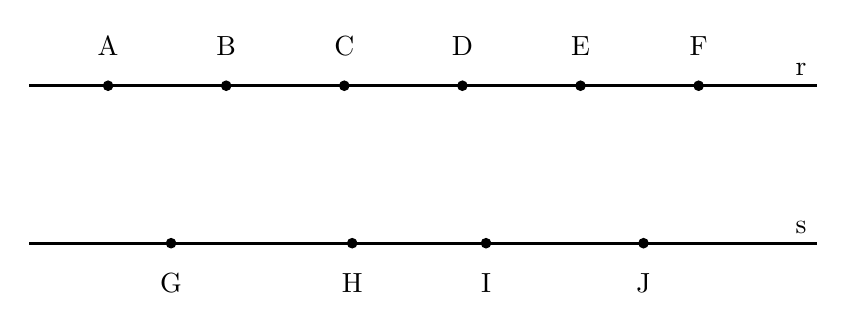
\begin{tikzpicture}
  \draw [very thick] (0,0)--(10,0);
  \draw [fill] (1,0) circle [radius = 0.06];\draw node  at (1,.5) {A};
  \draw [fill] (2.5,0) circle [radius = 0.06];\draw node  at (2.5,0.5) {B};
   \draw [fill] (4,0) circle [radius = 0.06];\draw node at (4,.5) {C};
   \draw [fill] (5.5,0) circle [radius = 0.06];\draw node at (5.5,.5) {D};
   \draw [fill] (7,0) circle [radius = 0.06];\draw node at (7,.5) {E};
   \draw [fill] (8.5,0) circle [radius = 0.06];\draw node at (8.5,.5) {F}; \draw node at (9.8,.2) {r};
    \draw [very thick] (0,-2)--(10,-2);
    \draw [fill] (1.8,-2) circle [radius = 0.06];\draw node at (1.8,-2.5) {G};
    \draw [fill] (4.1,-2) circle [radius = 0.06];\draw node at (4.1,-2.5) {H};
    \draw [fill] (5.8,-2) circle [radius = 0.06];\draw node at (5.8,-2.5) {I};
    \draw [fill] (7.8,-2) circle [radius = 0.06];\draw node at (7.8,-2.5) {J}; \draw node at (9.8,-1.8) {s};
  \end{tikzpicture}
\end{center}
   \begin{enumerate}[(a)]
   \item quantas retas ficam determinadas pelos 10 pontos A, B, C, D, E, F, G, H, I e J?
   \item quantos triângulos ficam determinados por esses 10 pontos distintos?   
   \item de todos os triângulos determinados por esses 10 pontos distintos, quantos tem como vértice o ponto H?
   \item de todos os triângulos determinados por esses 10 pontos distintos, quantos tem um lado contido na reta r?
   \item quantos quadriláteros convexos ficam determinados por esses 10 pontos distintos?
   \end{enumerate}
     \begin{sol}
        \phantom{A}
        \begin{enumerate} [(a)]
            \item $\mathrm{C}_{6,1}\cdot\mathrm{C}_{4,1}+2= 26$
            \item 2 pontos de r e 1 de s ou 1 ponto de r e 2 de s \\
            $\mathrm{C}_{6,2}\cdot \mathrm{C}_{4,1}+\mathrm{C}_{6,1}\cdot\mathrm{C}_{4,2}=96$
            \item $\mathrm{C}_{6,1}\cdot3+\mathrm{C}_{6,2}\cdot1=33$
            \item $\mathrm{C}_{4,1}\cdot\mathrm{C}_{6,2}=60$
            \item $\mathrm{C}_{6,2}\cdot\mathrm{C}_{4,2}=90$
        \end{enumerate}
     \end{sol}
\end{ex}